\begin{figure}[t]
\centering
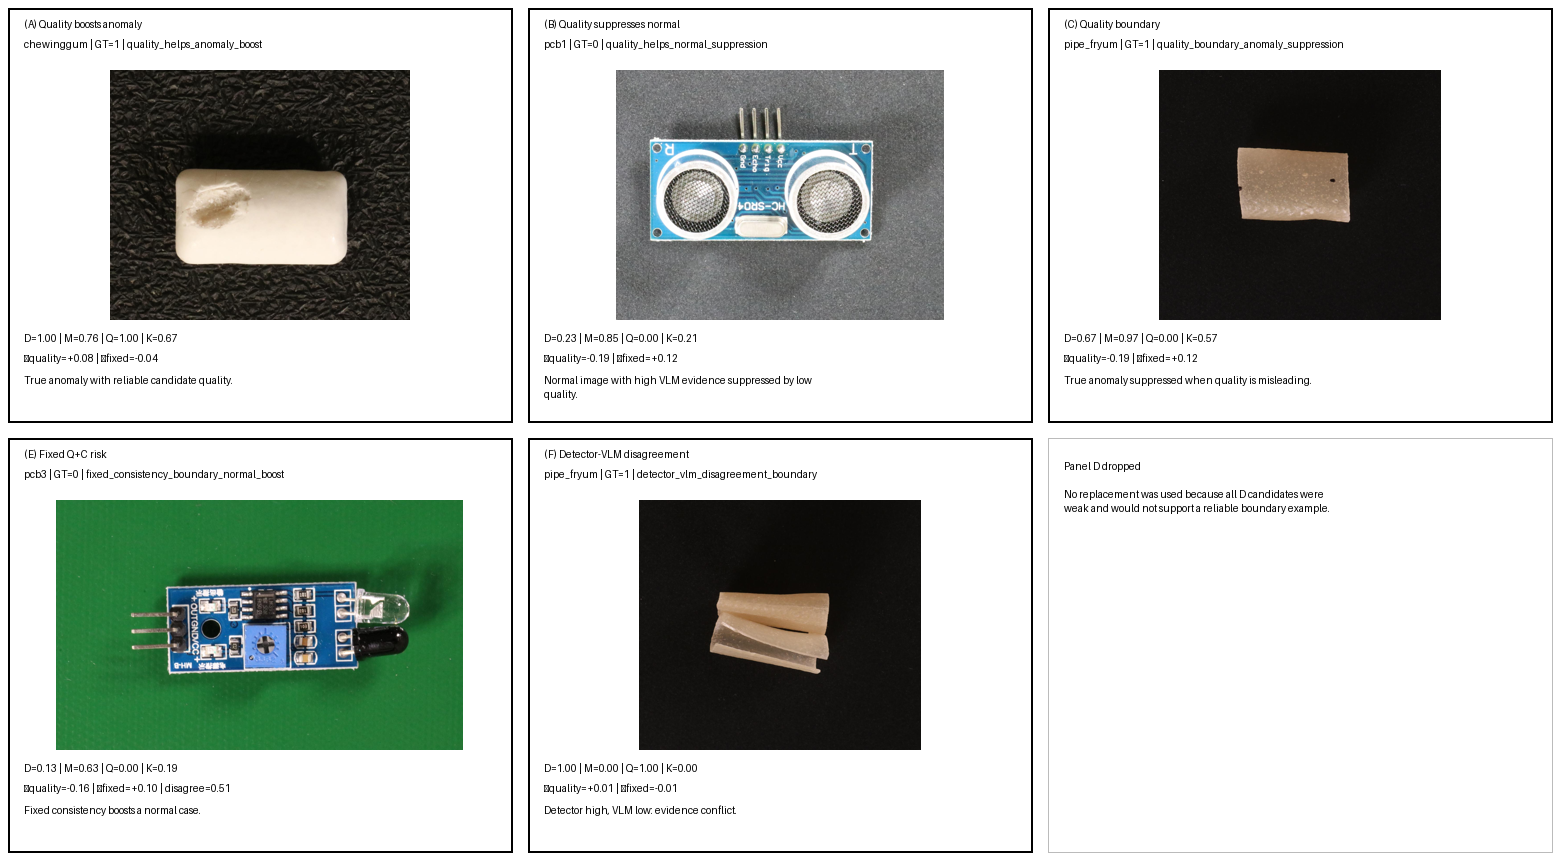
\includegraphics[width=\linewidth]{figures/figure2_boundary_cases_montage.png}
\caption{Representative boundary cases for quality-calibrated localization-guided VLM reasoning. Quality calibration can boost true anomaly evidence and suppress normal false positives, but it can also fail when candidate quality is misleading. Fixed Q+C can over-boost normal evidence, and detector-VLM disagreement remains a boundary case. These examples illustrate method boundaries rather than universal behavior.}
\label{fig:boundary_cases}
\end{figure}
